\documentclass[1p]{elsarticle_modified}
%\bibliographystyle{elsarticle-num}

%\usepackage[colorlinks]{hyperref}
%\usepackage{abbrmath_seonhwa} %\Abb, \Ascr, \Acal ,\Abf, \Afrak
\usepackage{amsfonts}
\usepackage{amssymb}
\usepackage{amsmath}
\usepackage{amsthm}
\usepackage{scalefnt}
\usepackage{amsbsy}
\usepackage{kotex}
\usepackage{caption}
\usepackage{subfig}
\usepackage{color}
\usepackage{graphicx}
\usepackage{xcolor} %% white, black, red, green, blue, cyan, magenta, yellow
\usepackage{float}
\usepackage{setspace}
\usepackage{hyperref}

\usepackage{tikz}
\usetikzlibrary{arrows}

\usepackage{multirow}
\usepackage{array} % fixed length table
\usepackage{hhline}

%%%%%%%%%%%%%%%%%%%%%
\makeatletter
\renewcommand*\env@matrix[1][\arraystretch]{%
	\edef\arraystretch{#1}%
	\hskip -\arraycolsep
	\let\@ifnextchar\new@ifnextchar
	\array{*\c@MaxMatrixCols c}}
\makeatother %https://tex.stackexchange.com/questions/14071/how-can-i-increase-the-line-spacing-in-a-matrix
%%%%%%%%%%%%%%%

\usepackage[normalem]{ulem}

\newcommand{\msout}[1]{\ifmmode\text{\sout{\ensuremath{#1}}}\else\sout{#1}\fi}
%SOURCE: \msout is \stkout macro in https://tex.stackexchange.com/questions/20609/strikeout-in-math-mode

\newcommand{\cancel}[1]{
	\ifmmode
	{\color{red}\msout{#1}}
	\else
	{\color{red}\sout{#1}}
	\fi
}

\newcommand{\add}[1]{
	{\color{blue}\uwave{#1}}
}

\newcommand{\replace}[2]{
	\ifmmode
	{\color{red}\msout{#1}}{\color{blue}\uwave{#2}}
	\else
	{\color{red}\sout{#1}}{\color{blue}\uwave{#2}}
	\fi
}

\newcommand{\Sol}{\mathcal{S}} %segment
\newcommand{\D}{D} %diagram
\newcommand{\A}{\mathcal{A}} %arc


%%%%%%%%%%%%%%%%%%%%%%%%%%%%%5 test

\def\sl{\operatorname{\textup{SL}}(2,\Cbb)}
\def\psl{\operatorname{\textup{PSL}}(2,\Cbb)}
\def\quan{\mkern 1mu \triangleright \mkern 1mu}

\theoremstyle{definition}
\newtheorem{thm}{Theorem}[section]
\newtheorem{prop}[thm]{Proposition}
\newtheorem{lem}[thm]{Lemma}
\newtheorem{ques}[thm]{Question}
\newtheorem{cor}[thm]{Corollary}
\newtheorem{defn}[thm]{Definition}
\newtheorem{exam}[thm]{Example}
\newtheorem{rmk}[thm]{Remark}
\newtheorem{alg}[thm]{Algorithm}

\newcommand{\I}{\sqrt{-1}}
\begin{document}

%\begin{frontmatter}
%
%\title{Boundary parabolic representations of knots up to 8 crossings}
%
%%% Group authors per affiliation:
%\author{Yunhi Cho} 
%\address{Department of Mathematics, University of Seoul, Seoul, Korea}
%\ead{yhcho@uos.ac.kr}
%
%
%\author{Seonhwa Kim} %\fnref{s_kim}}
%\address{Center for Geometry and Physics, Institute for Basic Science, Pohang, 37673, Korea}
%\ead{ryeona17@ibs.re.kr}
%
%\author{Hyuk Kim}
%\address{Department of Mathematical Sciences, Seoul National University, Seoul 08826, Korea}
%\ead{hyukkim@snu.ac.kr}
%
%\author{Seokbeom Yoon}
%\address{Department of Mathematical Sciences, Seoul National University, Seoul, 08826,  Korea}
%\ead{sbyoon15@snu.ac.kr}
%
%\begin{abstract}
%We find all boundary parabolic representation of knots up to 8 crossings.
%
%\end{abstract}
%\begin{keyword}
%    \MSC[2010] 57M25 
%\end{keyword}
%
%\end{frontmatter}

%\linenumbers
%\tableofcontents
%
\newcommand\colored[1]{\textcolor{white}{\rule[-0.35ex]{0.8em}{1.4ex}}\kern-0.8em\color{red} #1}%
%\newcommand\colored[1]{\textcolor{white}{ #1}\kern-2.17ex	\textcolor{white}{ #1}\kern-1.81ex	\textcolor{white}{ #1}\kern-2.15ex\color{red}#1	}

{\Large $\underline{12n_{0274}~(K12n_{0274})}$}

\setlength{\tabcolsep}{10pt}
\renewcommand{\arraystretch}{1.6}
\vspace{1cm}\begin{tabular}{m{100pt}>{\centering\arraybackslash}m{274pt}}
\multirow{5}{120pt}{
	\centering
	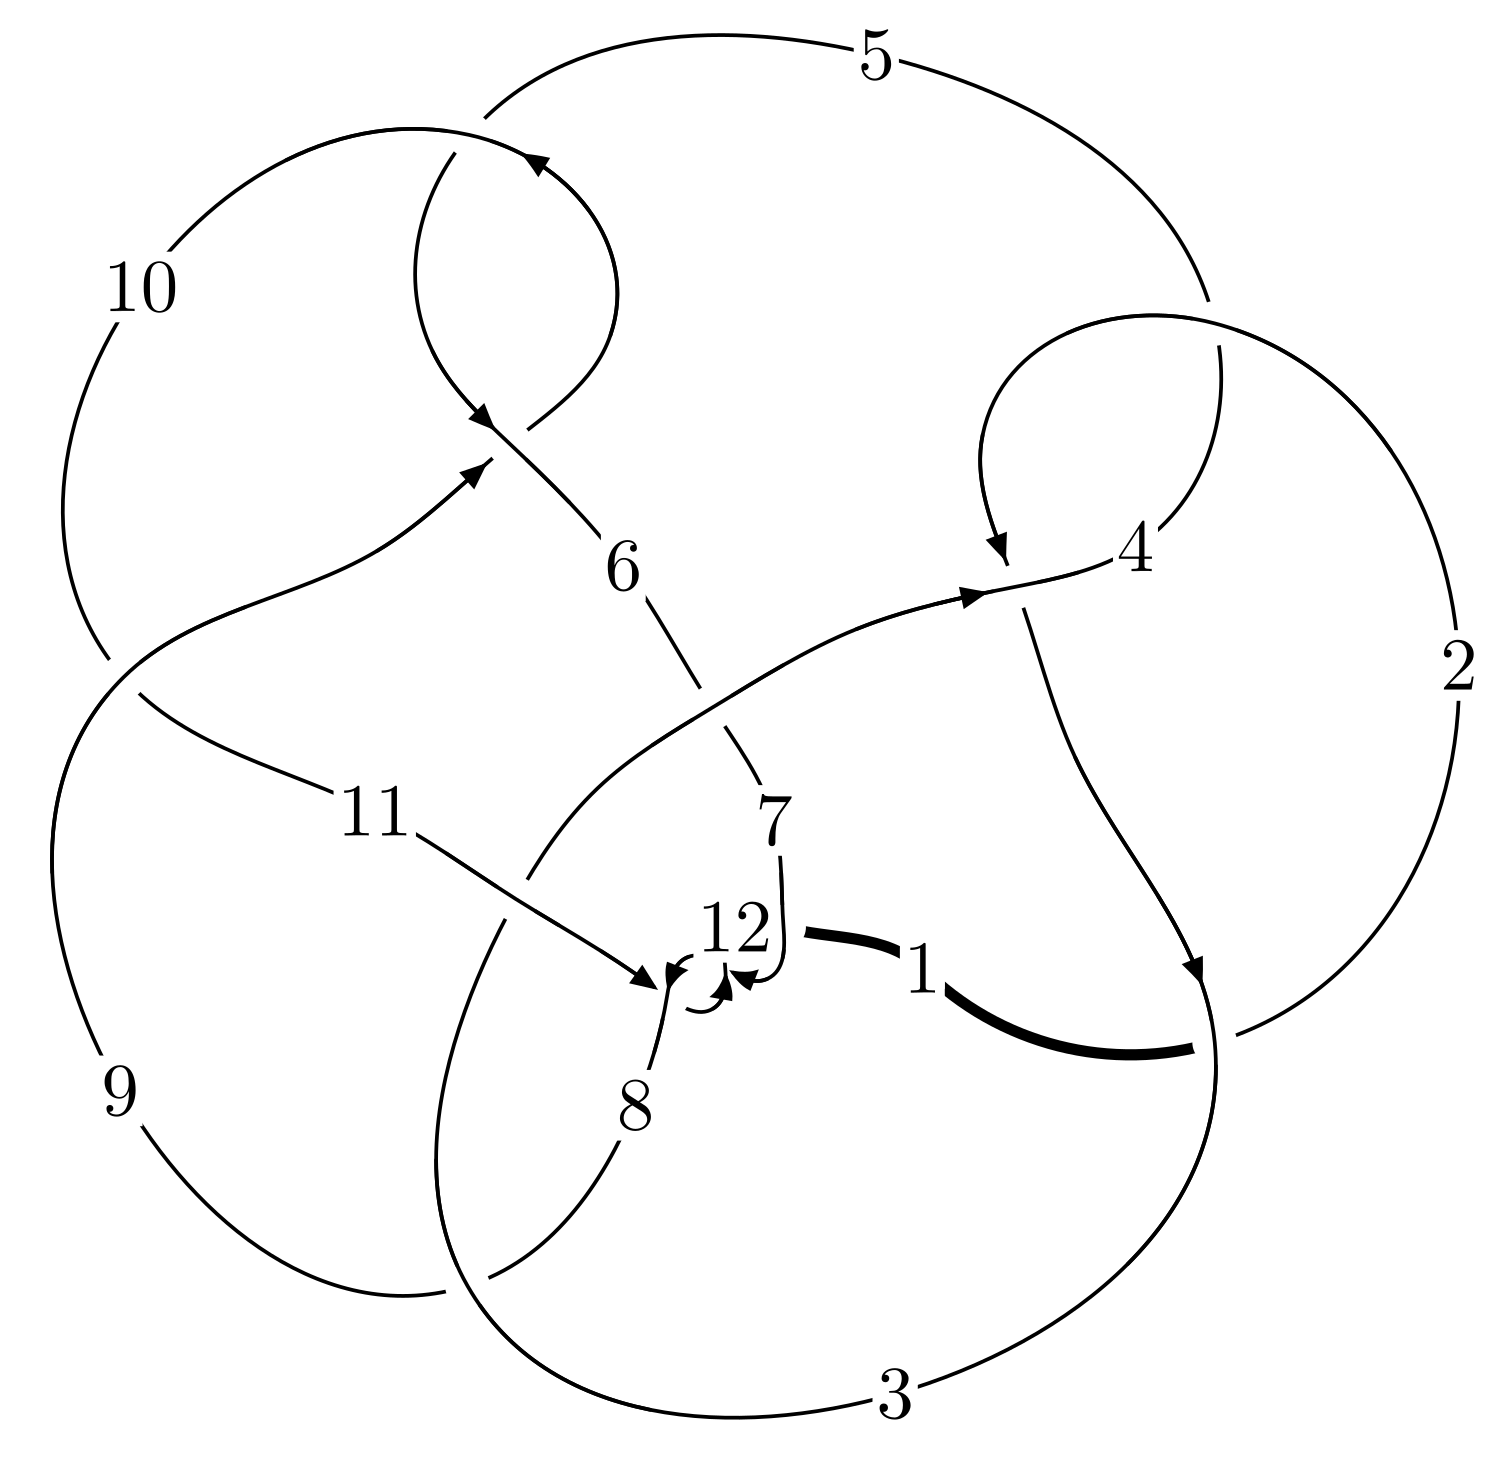
\includegraphics[width=112pt]{../../../GIT/diagram.site/Diagrams/png/2363_12n_0274.png}\\
\ \ \ A knot diagram\footnotemark}&
\allowdisplaybreaks
\textbf{Linearized knot diagam} \\
\cline{2-2}
 &
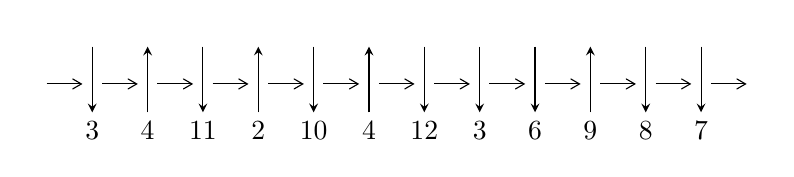
\begin{tikzpicture}[x=20pt, y=17pt]
	% nodes
	\node (C0) at (0, 0) {};
	\node (C1) at (1, 0) {};
	\node (C1U) at (1, +1) {};
	\node (C1D) at (1, -1) {3};

	\node (C2) at (2, 0) {};
	\node (C2U) at (2, +1) {};
	\node (C2D) at (2, -1) {4};

	\node (C3) at (3, 0) {};
	\node (C3U) at (3, +1) {};
	\node (C3D) at (3, -1) {11};

	\node (C4) at (4, 0) {};
	\node (C4U) at (4, +1) {};
	\node (C4D) at (4, -1) {2};

	\node (C5) at (5, 0) {};
	\node (C5U) at (5, +1) {};
	\node (C5D) at (5, -1) {10};

	\node (C6) at (6, 0) {};
	\node (C6U) at (6, +1) {};
	\node (C6D) at (6, -1) {4};

	\node (C7) at (7, 0) {};
	\node (C7U) at (7, +1) {};
	\node (C7D) at (7, -1) {12};

	\node (C8) at (8, 0) {};
	\node (C8U) at (8, +1) {};
	\node (C8D) at (8, -1) {3};

	\node (C9) at (9, 0) {};
	\node (C9U) at (9, +1) {};
	\node (C9D) at (9, -1) {6};

	\node (C10) at (10, 0) {};
	\node (C10U) at (10, +1) {};
	\node (C10D) at (10, -1) {9};

	\node (C11) at (11, 0) {};
	\node (C11U) at (11, +1) {};
	\node (C11D) at (11, -1) {8};

	\node (C12) at (12, 0) {};
	\node (C12U) at (12, +1) {};
	\node (C12D) at (12, -1) {7};
	\node (C13) at (13, 0) {};

	% arrows
	\draw[->,>={angle 60}]
	(C0) edge (C1) (C1) edge (C2) (C2) edge (C3) (C3) edge (C4) (C4) edge (C5) (C5) edge (C6) (C6) edge (C7) (C7) edge (C8) (C8) edge (C9) (C9) edge (C10) (C10) edge (C11) (C11) edge (C12) (C12) edge (C13) ;	\draw[->,>=stealth]
	(C1U) edge (C1D) (C2D) edge (C2U) (C3U) edge (C3D) (C4D) edge (C4U) (C5U) edge (C5D) (C6D) edge (C6U) (C7U) edge (C7D) (C8U) edge (C8D) (C9U) edge (C9D) (C10D) edge (C10U) (C11U) edge (C11D) (C12U) edge (C12D) ;
	\end{tikzpicture} \\
\hhline{~~} \\& 
\textbf{Solving Sequence} \\ \cline{2-2} 
 &
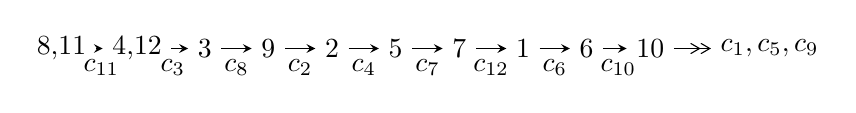
\begin{tikzpicture}[x=23pt, y=7pt]
	% node
	\node (A0) at (-1/8, 0) {8,11};
	\node (A1) at (17/16, 0) {4,12};
	\node (A2) at (17/8, 0) {3};
	\node (A3) at (25/8, 0) {9};
	\node (A4) at (33/8, 0) {2};
	\node (A5) at (41/8, 0) {5};
	\node (A6) at (49/8, 0) {7};
	\node (A7) at (57/8, 0) {1};
	\node (A8) at (65/8, 0) {6};
	\node (A9) at (73/8, 0) {10};
	\node (C1) at (1/2, -1) {$c_{11}$};
	\node (C2) at (13/8, -1) {$c_{3}$};
	\node (C3) at (21/8, -1) {$c_{8}$};
	\node (C4) at (29/8, -1) {$c_{2}$};
	\node (C5) at (37/8, -1) {$c_{4}$};
	\node (C6) at (45/8, -1) {$c_{7}$};
	\node (C7) at (53/8, -1) {$c_{12}$};
	\node (C8) at (61/8, -1) {$c_{6}$};
	\node (C9) at (69/8, -1) {$c_{10}$};
	\node (A10) at (11, 0) {$c_{1},c_{5},c_{9}$};

	% edge
	\draw[->,>=stealth]	
	(A0) edge (A1) (A1) edge (A2) (A2) edge (A3) (A3) edge (A4) (A4) edge (A5) (A5) edge (A6) (A6) edge (A7) (A7) edge (A8) (A8) edge (A9) ;
	\draw[->>,>={angle 60}]	
	(A9) edge (A10);
\end{tikzpicture} \\ 

\end{tabular} \\

\footnotetext{
The image of knot diagram is generated by the software ``\textbf{Draw programme}" developed by Andrew Bartholomew(\url{http://www.layer8.co.uk/maths/draw/index.htm\#Running-draw}), where we modified some parts for our purpose(\url{https://github.com/CATsTAILs/LinksPainter}).
}\phantom \\ \newline 
\centering \textbf{Ideals for irreducible components\footnotemark of $X_{\text{par}}$} 
 
\begin{align*}
I^u_{1}&=\langle 
- u^{12}+5 u^{11}-18 u^{10}+45 u^9-87 u^8+135 u^7-162 u^6+154 u^5-100 u^4+34 u^3+12 u^2+4 b-24 u+8,\\
\phantom{I^u_{1}}&\phantom{= \langle  }- u^{11}+5 u^{10}-18 u^9+41 u^8-75 u^7+103 u^6-110 u^5+86 u^4-36 u^3-2 u^2+4 a+20 u-12,\\
\phantom{I^u_{1}}&\phantom{= \langle  }u^{13}-5 u^{12}+18 u^{11}-45 u^{10}+89 u^9-141 u^8+178 u^7-180 u^6+134 u^5-64 u^4+4 u^3+24 u^2-16 u+4\rangle \\
I^u_{2}&=\langle 
- u^{11} a-2 u^{10} a+\cdots-2 a-3,\;3 u^{12} a- u^{12}+\cdots+2 a^2-2,\\
\phantom{I^u_{2}}&\phantom{= \langle  }u^{13}+2 u^{12}+7 u^{11}+10 u^{10}+18 u^9+20 u^8+21 u^7+20 u^6+11 u^5+10 u^4+u^3+4 u^2+2\rangle \\
I^u_{3}&=\langle 
- a u+9 b+4 a- u+4,\;2 a^2- a u+3 u+5,\;u^2+2\rangle \\
I^u_{4}&=\langle 
4 b+2 a+u+2,\;2 a^2+2 a u+5,\;u^2+2\rangle \\
\\
I^v_{1}&=\langle 
a,\;b^2- b+1,\;v+1\rangle \\
I^v_{2}&=\langle 
a,\;b+v-1,\;v^2- v+1\rangle \\
\end{align*}
\raggedright * 6 irreducible components of $\dim_{\mathbb{C}}=0$, with total 51 representations.\\
\footnotetext{All coefficients of polynomials are rational numbers. But the coefficients are sometimes approximated in decimal forms when there is not enough margin.}
\newpage
\renewcommand{\arraystretch}{1}
\centering \section*{I. $I^u_{1}= \langle - u^{12}+5 u^{11}+\cdots+4 b+8,\;- u^{11}+5 u^{10}+\cdots+4 a-12,\;u^{13}-5 u^{12}+\cdots-16 u+4 \rangle$}
\flushleft \textbf{(i) Arc colorings}\\
\begin{tabular}{m{7pt} m{180pt} m{7pt} m{180pt} }
\flushright $a_{8}=$&$\begin{pmatrix}0\\u\end{pmatrix}$ \\
\flushright $a_{11}=$&$\begin{pmatrix}1\\0\end{pmatrix}$ \\
\flushright $a_{4}=$&$\begin{pmatrix}\frac{1}{4} u^{11}-\frac{5}{4} u^{10}+\cdots-5 u+3\\\frac{1}{4} u^{12}-\frac{5}{4} u^{11}+\cdots+6 u-2\end{pmatrix}$ \\
\flushright $a_{12}=$&$\begin{pmatrix}1\\u^2\end{pmatrix}$ \\
\flushright $a_{3}=$&$\begin{pmatrix}\frac{1}{4} u^{12}- u^{11}+\cdots+u+1\\\frac{1}{4} u^{12}-\frac{5}{4} u^{11}+\cdots+6 u-2\end{pmatrix}$ \\
\flushright $a_{9}=$&$\begin{pmatrix}\frac{1}{4} u^{12}- u^{11}+\cdots+\frac{1}{2} u^2-2 u\\-\frac{1}{4} u^{12}+\frac{3}{4} u^{11}+\cdots- u+1\end{pmatrix}$ \\
\flushright $a_{2}=$&$\begin{pmatrix}\frac{1}{4} u^{12}-\frac{3}{2} u^{11}+\cdots+8 u-2\\-\frac{1}{4} u^{12}+\frac{5}{4} u^{11}+\cdots-4 u+1\end{pmatrix}$ \\
\flushright $a_{5}=$&$\begin{pmatrix}- u^{12}+5 u^{11}+\cdots-20 u+7\\u^4+2 u^2\end{pmatrix}$ \\
\flushright $a_{7}=$&$\begin{pmatrix}u\\u^3+u\end{pmatrix}$ \\
\flushright $a_{1}=$&$\begin{pmatrix}u^2+1\\u^4+2 u^2\end{pmatrix}$ \\
\flushright $a_{6}=$&$\begin{pmatrix}\frac{1}{2} u^{12}-\frac{9}{4} u^{11}+\cdots+10 u-4\\\frac{1}{4} u^{12}-\frac{5}{4} u^{11}+\cdots+4 u-1\end{pmatrix}$ \\
\flushright $a_{10}=$&$\begin{pmatrix}\frac{1}{2} u^{12}-\frac{5}{4} u^{11}+\cdots-\frac{1}{2} u^2+u\\\frac{1}{4} u^{12}-\frac{3}{4} u^{11}+\cdots-2 u^2+u\end{pmatrix}$\\&\end{tabular}
\flushleft \textbf{(ii) Obstruction class $= -1$}\\~\\
\flushleft \textbf{(iii) Cusp Shapes $= 2 u^{12}-7 u^{11}+25 u^{10}-55 u^9+106 u^8-159 u^7+190 u^6-185 u^5+117 u^4-42 u^3-22 u^2+42 u-14$}\\~\\
\newpage\renewcommand{\arraystretch}{1}
\flushleft \textbf{(iv) u-Polynomials at the component}\newline \\
\begin{tabular}{m{50pt}|m{274pt}}
Crossings & \hspace{64pt}u-Polynomials at each crossing \\
\hline $$\begin{aligned}c_{1}\end{aligned}$$&$\begin{aligned}
&u^{13}+19 u^{12}+\cdots+15 u-1
\end{aligned}$\\
\hline $$\begin{aligned}c_{2},c_{4},c_{10}\end{aligned}$$&$\begin{aligned}
&u^{13}-3 u^{12}+\cdots- u+1
\end{aligned}$\\
\hline $$\begin{aligned}c_{3},c_{5},c_{9}\end{aligned}$$&$\begin{aligned}
&u^{13}+u^{12}+2 u^{11}+u^{10}+6 u^9+4 u^8+8 u^7+3 u^6+8 u^5+4 u^3+u^2+u+1
\end{aligned}$\\
\hline $$\begin{aligned}c_{6}\end{aligned}$$&$\begin{aligned}
&u^{13}+u^{12}+\cdots+1321 u+181
\end{aligned}$\\
\hline $$\begin{aligned}c_{7},c_{11},c_{12}\end{aligned}$$&$\begin{aligned}
&u^{13}-5 u^{12}+\cdots-16 u+4
\end{aligned}$\\
\hline $$\begin{aligned}c_{8}\end{aligned}$$&$\begin{aligned}
&u^{13}- u^{12}+\cdots-39 u+11
\end{aligned}$\\
\hline
\end{tabular}\\~\\
\newpage\renewcommand{\arraystretch}{1}
\flushleft \textbf{(v) Riley Polynomials at the component}\newline \\
\begin{tabular}{m{50pt}|m{274pt}}
Crossings & \hspace{64pt}Riley Polynomials at each crossing \\
\hline $$\begin{aligned}c_{1}\end{aligned}$$&$\begin{aligned}
&y^{13}-61 y^{12}+\cdots+287 y-1
\end{aligned}$\\
\hline $$\begin{aligned}c_{2},c_{4},c_{10}\end{aligned}$$&$\begin{aligned}
&y^{13}+19 y^{12}+\cdots+15 y-1
\end{aligned}$\\
\hline $$\begin{aligned}c_{3},c_{5},c_{9}\end{aligned}$$&$\begin{aligned}
&y^{13}+3 y^{12}+\cdots- y-1
\end{aligned}$\\
\hline $$\begin{aligned}c_{6}\end{aligned}$$&$\begin{aligned}
&y^{13}+39 y^{12}+\cdots+2051655 y-32761
\end{aligned}$\\
\hline $$\begin{aligned}c_{7},c_{11},c_{12}\end{aligned}$$&$\begin{aligned}
&y^{13}+11 y^{12}+\cdots+64 y-16
\end{aligned}$\\
\hline $$\begin{aligned}c_{8}\end{aligned}$$&$\begin{aligned}
&y^{13}-13 y^{12}+\cdots+1191 y-121
\end{aligned}$\\
\hline
\end{tabular}\\~\\
\newpage\flushleft \textbf{(vi) Complex Volumes and Cusp Shapes}
$$\begin{array}{c|c|c}  
\text{Solutions to }I^u_{1}& \I (\text{vol} + \sqrt{-1}CS) & \text{Cusp shape}\\
 \hline 
\begin{aligned}
u &= \phantom{-}1.148130 + 0.133771 I \\
a &= -0.461030 + 0.761015 I \\
b &= -0.953736 - 1.010370 I\end{aligned}
 & -12.6764 - 7.1373 I & -6.57814 + 4.53811 I \\ \hline\begin{aligned}
u &= \phantom{-}1.148130 - 0.133771 I \\
a &= -0.461030 - 0.761015 I \\
b &= -0.953736 + 1.010370 I\end{aligned}
 & -12.6764 + 7.1373 I & -6.57814 - 4.53811 I \\ \hline\begin{aligned}
u &= \phantom{-}0.122498 + 1.377410 I \\
a &= -0.69924 + 2.04411 I \\
b &= -0.201153 - 0.911850 I\end{aligned}
 & \phantom{-}7.00880 - 3.27286 I & \phantom{-}6.62507 + 4.15467 I \\ \hline\begin{aligned}
u &= \phantom{-}0.122498 - 1.377410 I \\
a &= -0.69924 - 2.04411 I \\
b &= -0.201153 + 0.911850 I\end{aligned}
 & \phantom{-}7.00880 + 3.27286 I & \phantom{-}6.62507 - 4.15467 I \\ \hline\begin{aligned}
u &= -0.12567 + 1.42776 I \\
a &= -0.020580 - 1.032540 I \\
b &= -0.563900 + 0.510841 I\end{aligned}
 & \phantom{-}3.89768 + 2.33726 I & -4.18156 - 2.46985 I \\ \hline\begin{aligned}
u &= -0.12567 - 1.42776 I \\
a &= -0.020580 + 1.032540 I \\
b &= -0.563900 - 0.510841 I\end{aligned}
 & \phantom{-}3.89768 - 2.33726 I & -4.18156 + 2.46985 I \\ \hline\begin{aligned}
u &= -0.534170\phantom{ +0.000000I} \\
a &= \phantom{-}0.577891\phantom{ +0.000000I} \\
b &= \phantom{-}0.497979\phantom{ +0.000000I}\end{aligned}
 & -0.888404\phantom{ +0.000000I} & -11.3990\phantom{ +0.000000I} \\ \hline\begin{aligned}
u &= \phantom{-}0.67458 + 1.31287 I \\
a &= -0.656821 + 0.500993 I \\
b &= \phantom{-}0.999822 - 0.879885 I\end{aligned}
 & -9.09521 + 0.75227 I & -5.18637 - 1.36359 I \\ \hline\begin{aligned}
u &= \phantom{-}0.67458 - 1.31287 I \\
a &= -0.656821 - 0.500993 I \\
b &= \phantom{-}0.999822 + 0.879885 I\end{aligned}
 & -9.09521 - 0.75227 I & -5.18637 + 1.36359 I \\ \hline\begin{aligned}
u &= \phantom{-}0.420458 + 0.308747 I \\
a &= \phantom{-}1.11560 - 0.96767 I \\
b &= \phantom{-}0.108686 + 0.774322 I\end{aligned}
 & \phantom{-}1.70562 - 1.30597 I & \phantom{-}1.36439 + 5.54852 I\\
 \hline 
 \end{array}$$\newpage$$\begin{array}{c|c|c}  
\text{Solutions to }I^u_{1}& \I (\text{vol} + \sqrt{-1}CS) & \text{Cusp shape}\\
 \hline 
\begin{aligned}
u &= \phantom{-}0.420458 - 0.308747 I \\
a &= \phantom{-}1.11560 + 0.96767 I \\
b &= \phantom{-}0.108686 - 0.774322 I\end{aligned}
 & \phantom{-}1.70562 + 1.30597 I & \phantom{-}1.36439 - 5.54852 I \\ \hline\begin{aligned}
u &= \phantom{-}0.52709 + 1.45902 I \\
a &= \phantom{-}0.43312 - 1.92910 I \\
b &= \phantom{-}0.861292 + 1.076230 I\end{aligned}
 & -7.6681 - 13.1014 I & -3.34370 + 7.13870 I \\ \hline\begin{aligned}
u &= \phantom{-}0.52709 - 1.45902 I \\
a &= \phantom{-}0.43312 + 1.92910 I \\
b &= \phantom{-}0.861292 - 1.076230 I\end{aligned}
 & -7.6681 + 13.1014 I & -3.34370 - 7.13870 I\\
 \hline 
 \end{array}$$\newpage\newpage\renewcommand{\arraystretch}{1}
\centering \section*{II. $I^u_{2}= \langle - u^{11} a-2 u^{10} a+\cdots-2 a-3,\;3 u^{12} a- u^{12}+\cdots+2 a^2-2,\;u^{13}+2 u^{12}+\cdots+4 u^2+2 \rangle$}
\flushleft \textbf{(i) Arc colorings}\\
\begin{tabular}{m{7pt} m{180pt} m{7pt} m{180pt} }
\flushright $a_{8}=$&$\begin{pmatrix}0\\u\end{pmatrix}$ \\
\flushright $a_{11}=$&$\begin{pmatrix}1\\0\end{pmatrix}$ \\
\flushright $a_{4}=$&$\begin{pmatrix}a\\\frac{1}{2} u^{11} a+u^{10} a+\cdots+a+\frac{3}{2}\end{pmatrix}$ \\
\flushright $a_{12}=$&$\begin{pmatrix}1\\u^2\end{pmatrix}$ \\
\flushright $a_{3}=$&$\begin{pmatrix}\frac{1}{2} u^{11} a+u^{10} a+\cdots+2 a+\frac{3}{2}\\\frac{1}{2} u^{11} a+u^{10} a+\cdots+a+\frac{3}{2}\end{pmatrix}$ \\
\flushright $a_{9}=$&$\begin{pmatrix}-\frac{1}{2} u^{12} a-\frac{3}{2} u^{11} a+\cdots-3 u^2-\frac{5}{2} u\\-\frac{1}{2} u^{12} a+\frac{1}{2} u^{12}+\cdots+a+\frac{1}{2}\end{pmatrix}$ \\
\flushright $a_{2}=$&$\begin{pmatrix}-\frac{1}{2} u^{12} a+\frac{1}{4} u^{12}+\cdots+\frac{3}{2} a+\frac{5}{2}\\\frac{1}{2} u^{11} a+\frac{1}{2} u^{12}+\cdots+2 a-\frac{1}{2}\end{pmatrix}$ \\
\flushright $a_{5}=$&$\begin{pmatrix}u^{12}+u^{11}+\cdots+2 a-3\\u^4+2 u^2\end{pmatrix}$ \\
\flushright $a_{7}=$&$\begin{pmatrix}u\\u^3+u\end{pmatrix}$ \\
\flushright $a_{1}=$&$\begin{pmatrix}u^2+1\\u^4+2 u^2\end{pmatrix}$ \\
\flushright $a_{6}=$&$\begin{pmatrix}\frac{1}{2} u^{12} a+\frac{1}{2} u^{11}+\cdots-2 a+\frac{1}{2}\\\frac{1}{2} u^{11} a-\frac{1}{2} u^{12}+\cdots+2 a-\frac{5}{2}\end{pmatrix}$ \\
\flushright $a_{10}=$&$\begin{pmatrix}\frac{1}{2} u^{12} a-\frac{1}{4} u^{12}+\cdots+\frac{3}{2} a+\frac{5}{2}\\\frac{1}{2} u^{11} a+\frac{1}{2} u^{12}+\cdots+2 a+\frac{1}{2}\end{pmatrix}$\\&\end{tabular}
\flushleft \textbf{(ii) Obstruction class $= -1$}\\~\\
\flushleft \textbf{(iii) Cusp Shapes $= - u^{12}-3 u^{10}+4 u^9+2 u^8+14 u^7+15 u^6+12 u^5+17 u^4-2 u^3+7 u^2-6 u$}\\~\\
\newpage\renewcommand{\arraystretch}{1}
\flushleft \textbf{(iv) u-Polynomials at the component}\newline \\
\begin{tabular}{m{50pt}|m{274pt}}
Crossings & \hspace{64pt}u-Polynomials at each crossing \\
\hline $$\begin{aligned}c_{1}\end{aligned}$$&$\begin{aligned}
&u^{26}+30 u^{25}+\cdots-1609 u+81
\end{aligned}$\\
\hline $$\begin{aligned}c_{2},c_{4},c_{10}\end{aligned}$$&$\begin{aligned}
&u^{26}-6 u^{25}+\cdots-95 u+9
\end{aligned}$\\
\hline $$\begin{aligned}c_{3},c_{5},c_{9}\end{aligned}$$&$\begin{aligned}
&u^{26}+2 u^{25}+\cdots-5 u+3
\end{aligned}$\\
\hline $$\begin{aligned}c_{6}\end{aligned}$$&$\begin{aligned}
&u^{26}+3 u^{25}+\cdots-8726 u+1181
\end{aligned}$\\
\hline $$\begin{aligned}c_{7},c_{11},c_{12}\end{aligned}$$&$\begin{aligned}
&(u^{13}+2 u^{12}+\cdots+4 u^2+2)^{2}
\end{aligned}$\\
\hline $$\begin{aligned}c_{8}\end{aligned}$$&$\begin{aligned}
&u^{26}+u^{25}+\cdots-456 u+241
\end{aligned}$\\
\hline
\end{tabular}\\~\\
\newpage\renewcommand{\arraystretch}{1}
\flushleft \textbf{(v) Riley Polynomials at the component}\newline \\
\begin{tabular}{m{50pt}|m{274pt}}
Crossings & \hspace{64pt}Riley Polynomials at each crossing \\
\hline $$\begin{aligned}c_{1}\end{aligned}$$&$\begin{aligned}
&y^{26}-50 y^{25}+\cdots+5625167 y+6561
\end{aligned}$\\
\hline $$\begin{aligned}c_{2},c_{4},c_{10}\end{aligned}$$&$\begin{aligned}
&y^{26}+30 y^{25}+\cdots-1609 y+81
\end{aligned}$\\
\hline $$\begin{aligned}c_{3},c_{5},c_{9}\end{aligned}$$&$\begin{aligned}
&y^{26}+6 y^{25}+\cdots+95 y+9
\end{aligned}$\\
\hline $$\begin{aligned}c_{6}\end{aligned}$$&$\begin{aligned}
&y^{26}+37 y^{25}+\cdots-40866606 y+1394761
\end{aligned}$\\
\hline $$\begin{aligned}c_{7},c_{11},c_{12}\end{aligned}$$&$\begin{aligned}
&(y^{13}+10 y^{12}+\cdots-16 y-4)^{2}
\end{aligned}$\\
\hline $$\begin{aligned}c_{8}\end{aligned}$$&$\begin{aligned}
&y^{26}-15 y^{25}+\cdots-481230 y+58081
\end{aligned}$\\
\hline
\end{tabular}\\~\\
\newpage\flushleft \textbf{(vi) Complex Volumes and Cusp Shapes}
$$\begin{array}{c|c|c}  
\text{Solutions to }I^u_{2}& \I (\text{vol} + \sqrt{-1}CS) & \text{Cusp shape}\\
 \hline 
\begin{aligned}
u &= -0.190251 + 0.933207 I \\
a &= \phantom{-}0.298460 - 0.362265 I \\
b &= \phantom{-}0.719395 + 0.860977 I\end{aligned}
 & \phantom{-}1.31987 + 0.84014 I & -1.01632 - 1.58660 I \\ \hline\begin{aligned}
u &= -0.190251 + 0.933207 I \\
a &= -0.31610 - 2.95092 I \\
b &= -0.406685 + 1.088750 I\end{aligned}
 & \phantom{-}1.31987 + 0.84014 I & -1.01632 - 1.58660 I \\ \hline\begin{aligned}
u &= -0.190251 - 0.933207 I \\
a &= \phantom{-}0.298460 + 0.362265 I \\
b &= \phantom{-}0.719395 - 0.860977 I\end{aligned}
 & \phantom{-}1.31987 - 0.84014 I & -1.01632 + 1.58660 I \\ \hline\begin{aligned}
u &= -0.190251 - 0.933207 I \\
a &= -0.31610 + 2.95092 I \\
b &= -0.406685 - 1.088750 I\end{aligned}
 & \phantom{-}1.31987 - 0.84014 I & -1.01632 + 1.58660 I \\ \hline\begin{aligned}
u &= -0.522806 + 0.734222 I \\
a &= \phantom{-}0.408662 + 0.796811 I \\
b &= \phantom{-}0.798739 - 0.694333 I\end{aligned}
 & -1.83264 + 2.12437 I & -6.63093 - 3.54511 I \\ \hline\begin{aligned}
u &= -0.522806 + 0.734222 I \\
a &= \phantom{-}0.671809 - 0.426036 I \\
b &= -0.780847 - 0.269963 I\end{aligned}
 & -1.83264 + 2.12437 I & -6.63093 - 3.54511 I \\ \hline\begin{aligned}
u &= -0.522806 - 0.734222 I \\
a &= \phantom{-}0.408662 - 0.796811 I \\
b &= \phantom{-}0.798739 + 0.694333 I\end{aligned}
 & -1.83264 - 2.12437 I & -6.63093 + 3.54511 I \\ \hline\begin{aligned}
u &= -0.522806 - 0.734222 I \\
a &= \phantom{-}0.671809 + 0.426036 I \\
b &= -0.780847 + 0.269963 I\end{aligned}
 & -1.83264 - 2.12437 I & -6.63093 + 3.54511 I \\ \hline\begin{aligned}
u &= \phantom{-}0.354216 + 1.088690 I \\
a &= \phantom{-}0.804166 - 1.057380 I \\
b &= \phantom{-}0.780806 + 0.869479 I\end{aligned}
 & \phantom{-}1.27349 - 6.51495 I & -1.32958 + 6.90681 I \\ \hline\begin{aligned}
u &= \phantom{-}0.354216 + 1.088690 I \\
a &= -0.53542 + 2.66449 I \\
b &= -0.376849 - 1.157840 I\end{aligned}
 & \phantom{-}1.27349 - 6.51495 I & -1.32958 + 6.90681 I\\
 \hline 
 \end{array}$$\newpage$$\begin{array}{c|c|c}  
\text{Solutions to }I^u_{2}& \I (\text{vol} + \sqrt{-1}CS) & \text{Cusp shape}\\
 \hline 
\begin{aligned}
u &= \phantom{-}0.354216 - 1.088690 I \\
a &= \phantom{-}0.804166 + 1.057380 I \\
b &= \phantom{-}0.780806 - 0.869479 I\end{aligned}
 & \phantom{-}1.27349 + 6.51495 I & -1.32958 - 6.90681 I \\ \hline\begin{aligned}
u &= \phantom{-}0.354216 - 1.088690 I \\
a &= -0.53542 - 2.66449 I \\
b &= -0.376849 + 1.157840 I\end{aligned}
 & \phantom{-}1.27349 + 6.51495 I & -1.32958 - 6.90681 I \\ \hline\begin{aligned}
u &= -1.16445\phantom{ +0.000000I} \\
a &= -0.292211 + 0.542220 I \\
b &= -0.996994 - 0.942106 I\end{aligned}
 & -12.9066\phantom{ +0.000000I} & -6.99580\phantom{ +0.000000I} \\ \hline\begin{aligned}
u &= -1.16445\phantom{ +0.000000I} \\
a &= -0.292211 - 0.542220 I \\
b &= -0.996994 + 0.942106 I\end{aligned}
 & -12.9066\phantom{ +0.000000I} & -6.99580\phantom{ +0.000000I} \\ \hline\begin{aligned}
u &= \phantom{-}0.475729 + 0.397522 I \\
a &= \phantom{-}0.255684 + 0.929938 I \\
b &= \phantom{-}0.587541 - 0.997816 I\end{aligned}
 & -0.73347 + 3.14087 I & -5.81698 - 0.90558 I \\ \hline\begin{aligned}
u &= \phantom{-}0.475729 + 0.397522 I \\
a &= \phantom{-}0.907624 + 1.022940 I \\
b &= -0.603946 + 0.535433 I\end{aligned}
 & -0.73347 + 3.14087 I & -5.81698 - 0.90558 I \\ \hline\begin{aligned}
u &= \phantom{-}0.475729 - 0.397522 I \\
a &= \phantom{-}0.255684 - 0.929938 I \\
b &= \phantom{-}0.587541 + 0.997816 I\end{aligned}
 & -0.73347 - 3.14087 I & -5.81698 + 0.90558 I \\ \hline\begin{aligned}
u &= \phantom{-}0.475729 - 0.397522 I \\
a &= \phantom{-}0.907624 - 1.022940 I \\
b &= -0.603946 - 0.535433 I\end{aligned}
 & -0.73347 - 3.14087 I & -5.81698 + 0.90558 I \\ \hline\begin{aligned}
u &= \phantom{-}0.065416 + 1.409480 I \\
a &= -0.944118 + 0.771575 I \\
b &= -0.110601 - 0.414458 I\end{aligned}
 & \phantom{-}5.12373 + 1.84437 I & \phantom{-}0.90018 - 3.35466 I \\ \hline\begin{aligned}
u &= \phantom{-}0.065416 + 1.409480 I \\
a &= \phantom{-}0.14726 - 1.84752 I \\
b &= -0.534312 + 0.945546 I\end{aligned}
 & \phantom{-}5.12373 + 1.84437 I & \phantom{-}0.90018 - 3.35466 I\\
 \hline 
 \end{array}$$\newpage$$\begin{array}{c|c|c}  
\text{Solutions to }I^u_{2}& \I (\text{vol} + \sqrt{-1}CS) & \text{Cusp shape}\\
 \hline 
\begin{aligned}
u &= \phantom{-}0.065416 - 1.409480 I \\
a &= -0.944118 - 0.771575 I \\
b &= -0.110601 + 0.414458 I\end{aligned}
 & \phantom{-}5.12373 - 1.84437 I & \phantom{-}0.90018 + 3.35466 I \\ \hline\begin{aligned}
u &= \phantom{-}0.065416 - 1.409480 I \\
a &= \phantom{-}0.14726 + 1.84752 I \\
b &= -0.534312 - 0.945546 I\end{aligned}
 & \phantom{-}5.12373 - 1.84437 I & \phantom{-}0.90018 + 3.35466 I \\ \hline\begin{aligned}
u &= -0.60008 + 1.40135 I \\
a &= -0.751907 - 0.379224 I \\
b &= \phantom{-}1.015400 + 0.803176 I\end{aligned}
 & -8.56727 + 6.23778 I & -4.60847 - 2.87458 I \\ \hline\begin{aligned}
u &= -0.60008 + 1.40135 I \\
a &= \phantom{-}0.34609 + 1.75574 I \\
b &= \phantom{-}0.908351 - 1.039740 I\end{aligned}
 & -8.56727 + 6.23778 I & -4.60847 - 2.87458 I \\ \hline\begin{aligned}
u &= -0.60008 - 1.40135 I \\
a &= -0.751907 + 0.379224 I \\
b &= \phantom{-}1.015400 - 0.803176 I\end{aligned}
 & -8.56727 - 6.23778 I & -4.60847 + 2.87458 I \\ \hline\begin{aligned}
u &= -0.60008 - 1.40135 I \\
a &= \phantom{-}0.34609 - 1.75574 I \\
b &= \phantom{-}0.908351 + 1.039740 I\end{aligned}
 & -8.56727 - 6.23778 I & -4.60847 + 2.87458 I\\
 \hline 
 \end{array}$$\newpage\newpage\renewcommand{\arraystretch}{1}
\centering \section*{III. $I^u_{3}= \langle - a u+9 b+4 a- u+4,\;2 a^2- a u+3 u+5,\;u^2+2 \rangle$}
\flushleft \textbf{(i) Arc colorings}\\
\begin{tabular}{m{7pt} m{180pt} m{7pt} m{180pt} }
\flushright $a_{8}=$&$\begin{pmatrix}0\\u\end{pmatrix}$ \\
\flushright $a_{11}=$&$\begin{pmatrix}1\\0\end{pmatrix}$ \\
\flushright $a_{4}=$&$\begin{pmatrix}a\\\frac{1}{9} a u-\frac{4}{9} a+\frac{1}{9} u-\frac{4}{9}\end{pmatrix}$ \\
\flushright $a_{12}=$&$\begin{pmatrix}1\\-2\end{pmatrix}$ \\
\flushright $a_{3}=$&$\begin{pmatrix}\frac{1}{9} a u+\frac{5}{9} a+\frac{1}{9} u-\frac{4}{9}\\\frac{1}{9} a u-\frac{4}{9} a+\frac{1}{9} u-\frac{4}{9}\end{pmatrix}$ \\
\flushright $a_{9}=$&$\begin{pmatrix}\frac{2}{3} a u+\frac{1}{3} a+\frac{1}{6} u-\frac{5}{3}\\\frac{1}{9} a u-\frac{4}{9} a+\frac{1}{9} u+\frac{5}{9}\end{pmatrix}$ \\
\flushright $a_{2}=$&$\begin{pmatrix}\frac{2}{9} a u+\frac{1}{9} a-\frac{5}{18} u-\frac{17}{9}\\\frac{1}{9} a u-\frac{4}{9} a+\frac{1}{9} u+\frac{5}{9}\end{pmatrix}$ \\
\flushright $a_{5}=$&$\begin{pmatrix}1\\0\end{pmatrix}$ \\
\flushright $a_{7}=$&$\begin{pmatrix}u\\- u\end{pmatrix}$ \\
\flushright $a_{1}=$&$\begin{pmatrix}-1\\0\end{pmatrix}$ \\
\flushright $a_{6}=$&$\begin{pmatrix}-\frac{5}{9} a u-\frac{7}{9} a-\frac{1}{18} u+\frac{20}{9}\\-\frac{1}{9} a u+\frac{4}{9} a-\frac{1}{9} u-\frac{5}{9}\end{pmatrix}$ \\
\flushright $a_{10}=$&$\begin{pmatrix}a+u\\\frac{1}{9} a u-\frac{4}{9} a+\frac{1}{9} u-\frac{4}{9}\end{pmatrix}$\\&\end{tabular}
\flushleft \textbf{(ii) Obstruction class $= 1$}\\~\\
\flushleft \textbf{(iii) Cusp Shapes $= -\frac{8}{9} a u+\frac{32}{9} a-\frac{8}{9} u-\frac{4}{9}$}\\~\\
\newpage\renewcommand{\arraystretch}{1}
\flushleft \textbf{(iv) u-Polynomials at the component}\newline \\
\begin{tabular}{m{50pt}|m{274pt}}
Crossings & \hspace{64pt}u-Polynomials at each crossing \\
\hline $$\begin{aligned}c_{1},c_{3},c_{4}\\c_{9},c_{10}\end{aligned}$$&$\begin{aligned}
&(u^2- u+1)^2
\end{aligned}$\\
\hline $$\begin{aligned}c_{2},c_{5}\end{aligned}$$&$\begin{aligned}
&(u^2+u+1)^2
\end{aligned}$\\
\hline $$\begin{aligned}c_{6}\end{aligned}$$&$\begin{aligned}
&u^4+2 u^3+u^2-6 u+3
\end{aligned}$\\
\hline $$\begin{aligned}c_{7},c_{11},c_{12}\end{aligned}$$&$\begin{aligned}
&(u^2+2)^2
\end{aligned}$\\
\hline $$\begin{aligned}c_{8}\end{aligned}$$&$\begin{aligned}
&u^4-2 u^3+u^2+6 u+3
\end{aligned}$\\
\hline
\end{tabular}\\~\\
\newpage\renewcommand{\arraystretch}{1}
\flushleft \textbf{(v) Riley Polynomials at the component}\newline \\
\begin{tabular}{m{50pt}|m{274pt}}
Crossings & \hspace{64pt}Riley Polynomials at each crossing \\
\hline $$\begin{aligned}c_{1},c_{2},c_{3}\\c_{4},c_{5},c_{9}\\c_{10}\end{aligned}$$&$\begin{aligned}
&(y^2+y+1)^2
\end{aligned}$\\
\hline $$\begin{aligned}c_{6},c_{8}\end{aligned}$$&$\begin{aligned}
&y^4-2 y^3+31 y^2-30 y+9
\end{aligned}$\\
\hline $$\begin{aligned}c_{7},c_{11},c_{12}\end{aligned}$$&$\begin{aligned}
&(y+2)^4
\end{aligned}$\\
\hline
\end{tabular}\\~\\
\newpage\flushleft \textbf{(vi) Complex Volumes and Cusp Shapes}
$$\begin{array}{c|c|c}  
\text{Solutions to }I^u_{3}& \I (\text{vol} + \sqrt{-1}CS) & \text{Cusp shape}\\
 \hline 
\begin{aligned}
u &= \phantom{-0.000000 -}1.414210 I \\
a &= \phantom{-}0.61237 - 1.37850 I \\
b &= -0.500000 + 0.866025 I\end{aligned}
 & \phantom{-}4.93480 + 4.05977 I & \phantom{-0.000000 } 0. - 6.92820 I \\ \hline\begin{aligned}
u &= \phantom{-0.000000 -}1.414210 I \\
a &= -0.61237 + 2.08560 I \\
b &= -0.500000 - 0.866025 I\end{aligned}
 & \phantom{-}4.93480 - 4.05977 I & \phantom{-0.000000 -}0. + 6.92820 I \\ \hline\begin{aligned}
u &= \phantom{-0.000000 } -1.414210 I \\
a &= \phantom{-}0.61237 + 1.37850 I \\
b &= -0.500000 - 0.866025 I\end{aligned}
 & \phantom{-}4.93480 - 4.05977 I & \phantom{-0.000000 -}0. + 6.92820 I \\ \hline\begin{aligned}
u &= \phantom{-0.000000 } -1.414210 I \\
a &= -0.61237 - 2.08560 I \\
b &= -0.500000 + 0.866025 I\end{aligned}
 & \phantom{-}4.93480 + 4.05977 I & \phantom{-0.000000 } 0. - 6.92820 I\\
 \hline 
 \end{array}$$\newpage\newpage\renewcommand{\arraystretch}{1}
\centering \section*{IV. $I^u_{4}= \langle 4 b+2 a+u+2,\;2 a^2+2 a u+5,\;u^2+2 \rangle$}
\flushleft \textbf{(i) Arc colorings}\\
\begin{tabular}{m{7pt} m{180pt} m{7pt} m{180pt} }
\flushright $a_{8}=$&$\begin{pmatrix}0\\u\end{pmatrix}$ \\
\flushright $a_{11}=$&$\begin{pmatrix}1\\0\end{pmatrix}$ \\
\flushright $a_{4}=$&$\begin{pmatrix}a\\-\frac{1}{2} a-\frac{1}{4} u-\frac{1}{2}\end{pmatrix}$ \\
\flushright $a_{12}=$&$\begin{pmatrix}1\\-2\end{pmatrix}$ \\
\flushright $a_{3}=$&$\begin{pmatrix}\frac{1}{2} a-\frac{1}{4} u-\frac{1}{2}\\-\frac{1}{2} a-\frac{1}{4} u-\frac{1}{2}\end{pmatrix}$ \\
\flushright $a_{9}=$&$\begin{pmatrix}\frac{1}{2} a u- a+\frac{1}{2} u+\frac{1}{2}\\\frac{1}{2} a+\frac{1}{4} u+\frac{1}{2}\end{pmatrix}$ \\
\flushright $a_{2}=$&$\begin{pmatrix}-\frac{1}{4} a u-\frac{1}{4} u-\frac{7}{4}\\-\frac{1}{2} a-\frac{1}{4} u+\frac{1}{2}\end{pmatrix}$ \\
\flushright $a_{5}=$&$\begin{pmatrix}1\\0\end{pmatrix}$ \\
\flushright $a_{7}=$&$\begin{pmatrix}u\\- u\end{pmatrix}$ \\
\flushright $a_{1}=$&$\begin{pmatrix}-1\\0\end{pmatrix}$ \\
\flushright $a_{6}=$&$\begin{pmatrix}-\frac{1}{2} a u+\frac{3}{2} a-\frac{1}{4} u\\-\frac{1}{2} a-\frac{1}{4} u-\frac{1}{2}\end{pmatrix}$ \\
\flushright $a_{10}=$&$\begin{pmatrix}\frac{3}{4} a u-\frac{1}{4} u+\frac{9}{4}\\\frac{1}{2} a+\frac{1}{4} u-\frac{1}{2}\end{pmatrix}$\\&\end{tabular}
\flushleft \textbf{(ii) Obstruction class $= 1$}\\~\\
\flushleft \textbf{(iii) Cusp Shapes $= 0$}\\~\\
\newpage\renewcommand{\arraystretch}{1}
\flushleft \textbf{(iv) u-Polynomials at the component}\newline \\
\begin{tabular}{m{50pt}|m{274pt}}
Crossings & \hspace{64pt}u-Polynomials at each crossing \\
\hline $$\begin{aligned}c_{1},c_{3},c_{4}\\c_{9},c_{10}\end{aligned}$$&$\begin{aligned}
&(u^2- u+1)^2
\end{aligned}$\\
\hline $$\begin{aligned}c_{2},c_{5}\end{aligned}$$&$\begin{aligned}
&(u^2+u+1)^2
\end{aligned}$\\
\hline $$\begin{aligned}c_{6}\end{aligned}$$&$\begin{aligned}
&u^4-4 u^3+4 u^2+3
\end{aligned}$\\
\hline $$\begin{aligned}c_{7},c_{11},c_{12}\end{aligned}$$&$\begin{aligned}
&(u^2+2)^2
\end{aligned}$\\
\hline $$\begin{aligned}c_{8}\end{aligned}$$&$\begin{aligned}
&u^4+4 u^3+4 u^2+3
\end{aligned}$\\
\hline
\end{tabular}\\~\\
\newpage\renewcommand{\arraystretch}{1}
\flushleft \textbf{(v) Riley Polynomials at the component}\newline \\
\begin{tabular}{m{50pt}|m{274pt}}
Crossings & \hspace{64pt}Riley Polynomials at each crossing \\
\hline $$\begin{aligned}c_{1},c_{2},c_{3}\\c_{4},c_{5},c_{9}\\c_{10}\end{aligned}$$&$\begin{aligned}
&(y^2+y+1)^2
\end{aligned}$\\
\hline $$\begin{aligned}c_{6},c_{8}\end{aligned}$$&$\begin{aligned}
&y^4-8 y^3+22 y^2+24 y+9
\end{aligned}$\\
\hline $$\begin{aligned}c_{7},c_{11},c_{12}\end{aligned}$$&$\begin{aligned}
&(y+2)^4
\end{aligned}$\\
\hline
\end{tabular}\\~\\
\newpage\flushleft \textbf{(vi) Complex Volumes and Cusp Shapes}
$$\begin{array}{c|c|c}  
\text{Solutions to }I^u_{4}& \I (\text{vol} + \sqrt{-1}CS) & \text{Cusp shape}\\
 \hline 
\begin{aligned}
u &= \phantom{-0.000000 -}1.414210 I \\
a &= \phantom{-0.000000 -}1.024940 I \\
b &= -0.500000 - 0.866025 I\end{aligned}
 & \phantom{-}4.93480\phantom{ +0.000000I} & \phantom{-0.000000 } 0 \\ \hline\begin{aligned}
u &= \phantom{-0.000000 -}1.414210 I \\
a &= \phantom{-0.000000 } -2.43916 I \\
b &= -0.500000 + 0.866025 I\end{aligned}
 & \phantom{-}4.93480\phantom{ +0.000000I} & \phantom{-0.000000 } 0 \\ \hline\begin{aligned}
u &= \phantom{-0.000000 } -1.414210 I \\
a &= \phantom{-0.000000 } -1.024940 I \\
b &= -0.500000 + 0.866025 I\end{aligned}
 & \phantom{-}4.93480\phantom{ +0.000000I} & \phantom{-0.000000 } 0 \\ \hline\begin{aligned}
u &= \phantom{-0.000000 } -1.414210 I \\
a &= \phantom{-0.000000 -}2.43916 I \\
b &= -0.500000 - 0.866025 I\end{aligned}
 & \phantom{-}4.93480\phantom{ +0.000000I} & \phantom{-0.000000 } 0\\
 \hline 
 \end{array}$$\newpage\newpage\renewcommand{\arraystretch}{1}
\centering \section*{V. $I^v_{1}= \langle a,\;b^2- b+1,\;v+1 \rangle$}
\flushleft \textbf{(i) Arc colorings}\\
\begin{tabular}{m{7pt} m{180pt} m{7pt} m{180pt} }
\flushright $a_{8}=$&$\begin{pmatrix}-1\\0\end{pmatrix}$ \\
\flushright $a_{11}=$&$\begin{pmatrix}1\\0\end{pmatrix}$ \\
\flushright $a_{4}=$&$\begin{pmatrix}0\\b\end{pmatrix}$ \\
\flushright $a_{12}=$&$\begin{pmatrix}1\\0\end{pmatrix}$ \\
\flushright $a_{3}=$&$\begin{pmatrix}b\\b\end{pmatrix}$ \\
\flushright $a_{9}=$&$\begin{pmatrix}- b\\- b+1\end{pmatrix}$ \\
\flushright $a_{2}=$&$\begin{pmatrix}b\\b-1\end{pmatrix}$ \\
\flushright $a_{5}=$&$\begin{pmatrix}-1\\0\end{pmatrix}$ \\
\flushright $a_{7}=$&$\begin{pmatrix}-1\\0\end{pmatrix}$ \\
\flushright $a_{1}=$&$\begin{pmatrix}1\\0\end{pmatrix}$ \\
\flushright $a_{6}=$&$\begin{pmatrix}-1\\- b+1\end{pmatrix}$ \\
\flushright $a_{10}=$&$\begin{pmatrix}0\\- b\end{pmatrix}$\\&\end{tabular}
\flushleft \textbf{(ii) Obstruction class $= 1$}\\~\\
\flushleft \textbf{(iii) Cusp Shapes $= 8 b-4$}\\~\\
\newpage\renewcommand{\arraystretch}{1}
\flushleft \textbf{(iv) u-Polynomials at the component}\newline \\
\begin{tabular}{m{50pt}|m{274pt}}
Crossings & \hspace{64pt}u-Polynomials at each crossing \\
\hline $$\begin{aligned}c_{1},c_{4},c_{5}\\c_{10}\end{aligned}$$&$\begin{aligned}
&u^2- u+1
\end{aligned}$\\
\hline $$\begin{aligned}c_{2},c_{3},c_{6}\\c_{8},c_{9}\end{aligned}$$&$\begin{aligned}
&u^2+u+1
\end{aligned}$\\
\hline $$\begin{aligned}c_{7},c_{11},c_{12}\end{aligned}$$&$\begin{aligned}
&u^2
\end{aligned}$\\
\hline
\end{tabular}\\~\\
\newpage\renewcommand{\arraystretch}{1}
\flushleft \textbf{(v) Riley Polynomials at the component}\newline \\
\begin{tabular}{m{50pt}|m{274pt}}
Crossings & \hspace{64pt}Riley Polynomials at each crossing \\
\hline $$\begin{aligned}c_{1},c_{2},c_{3}\\c_{4},c_{5},c_{6}\\c_{8},c_{9},c_{10}\end{aligned}$$&$\begin{aligned}
&y^2+y+1
\end{aligned}$\\
\hline $$\begin{aligned}c_{7},c_{11},c_{12}\end{aligned}$$&$\begin{aligned}
&y^2
\end{aligned}$\\
\hline
\end{tabular}\\~\\
\newpage\flushleft \textbf{(vi) Complex Volumes and Cusp Shapes}
$$\begin{array}{c|c|c}  
\text{Solutions to }I^v_{1}& \I (\text{vol} + \sqrt{-1}CS) & \text{Cusp shape}\\
 \hline 
\begin{aligned}
v &= -1.00000\phantom{ +0.000000I} \\
a &= \phantom{-0.000000 } 0 \\
b &= \phantom{-}0.500000 + 0.866025 I\end{aligned}
 & \phantom{-0.000000 } -4.05977 I & \phantom{-0.000000 -}0. + 6.92820 I \\ \hline\begin{aligned}
v &= -1.00000\phantom{ +0.000000I} \\
a &= \phantom{-0.000000 } 0 \\
b &= \phantom{-}0.500000 - 0.866025 I\end{aligned}
 & \phantom{-0.000000 -}4.05977 I & \phantom{-0.000000 } 0. - 6.92820 I\\
 \hline 
 \end{array}$$\newpage\newpage\renewcommand{\arraystretch}{1}
\centering \section*{VI. $I^v_{2}= \langle a,\;b+v-1,\;v^2- v+1 \rangle$}
\flushleft \textbf{(i) Arc colorings}\\
\begin{tabular}{m{7pt} m{180pt} m{7pt} m{180pt} }
\flushright $a_{8}=$&$\begin{pmatrix}v\\0\end{pmatrix}$ \\
\flushright $a_{11}=$&$\begin{pmatrix}1\\0\end{pmatrix}$ \\
\flushright $a_{4}=$&$\begin{pmatrix}0\\- v+1\end{pmatrix}$ \\
\flushright $a_{12}=$&$\begin{pmatrix}1\\0\end{pmatrix}$ \\
\flushright $a_{3}=$&$\begin{pmatrix}- v+1\\- v+1\end{pmatrix}$ \\
\flushright $a_{9}=$&$\begin{pmatrix}1\\- v+1\end{pmatrix}$ \\
\flushright $a_{2}=$&$\begin{pmatrix}- v+1\\- v\end{pmatrix}$ \\
\flushright $a_{5}=$&$\begin{pmatrix}-1\\0\end{pmatrix}$ \\
\flushright $a_{7}=$&$\begin{pmatrix}v\\0\end{pmatrix}$ \\
\flushright $a_{1}=$&$\begin{pmatrix}1\\0\end{pmatrix}$ \\
\flushright $a_{6}=$&$\begin{pmatrix}v\\- v+1\end{pmatrix}$ \\
\flushright $a_{10}=$&$\begin{pmatrix}- v+2\\- v\end{pmatrix}$\\&\end{tabular}
\flushleft \textbf{(ii) Obstruction class $= 1$}\\~\\
\flushleft \textbf{(iii) Cusp Shapes $= -6$}\\~\\
\newpage\renewcommand{\arraystretch}{1}
\flushleft \textbf{(iv) u-Polynomials at the component}\newline \\
\begin{tabular}{m{50pt}|m{274pt}}
Crossings & \hspace{64pt}u-Polynomials at each crossing \\
\hline $$\begin{aligned}c_{1},c_{4},c_{5}\\c_{10}\end{aligned}$$&$\begin{aligned}
&u^2- u+1
\end{aligned}$\\
\hline $$\begin{aligned}c_{2},c_{3},c_{9}\end{aligned}$$&$\begin{aligned}
&u^2+u+1
\end{aligned}$\\
\hline $$\begin{aligned}c_{6},c_{8}\end{aligned}$$&$\begin{aligned}
&(u-1)^2
\end{aligned}$\\
\hline $$\begin{aligned}c_{7},c_{11},c_{12}\end{aligned}$$&$\begin{aligned}
&u^2
\end{aligned}$\\
\hline
\end{tabular}\\~\\
\newpage\renewcommand{\arraystretch}{1}
\flushleft \textbf{(v) Riley Polynomials at the component}\newline \\
\begin{tabular}{m{50pt}|m{274pt}}
Crossings & \hspace{64pt}Riley Polynomials at each crossing \\
\hline $$\begin{aligned}c_{1},c_{2},c_{3}\\c_{4},c_{5},c_{9}\\c_{10}\end{aligned}$$&$\begin{aligned}
&y^2+y+1
\end{aligned}$\\
\hline $$\begin{aligned}c_{6},c_{8}\end{aligned}$$&$\begin{aligned}
&(y-1)^2
\end{aligned}$\\
\hline $$\begin{aligned}c_{7},c_{11},c_{12}\end{aligned}$$&$\begin{aligned}
&y^2
\end{aligned}$\\
\hline
\end{tabular}\\~\\
\newpage\flushleft \textbf{(vi) Complex Volumes and Cusp Shapes}
$$\begin{array}{c|c|c}  
\text{Solutions to }I^v_{2}& \I (\text{vol} + \sqrt{-1}CS) & \text{Cusp shape}\\
 \hline 
\begin{aligned}
v &= \phantom{-}0.500000 + 0.866025 I \\
a &= \phantom{-0.000000 } 0 \\
b &= \phantom{-}0.500000 - 0.866025 I\end{aligned}
 & \phantom{-0.000000 } 0 & -6.00000\phantom{ +0.000000I} \\ \hline\begin{aligned}
v &= \phantom{-}0.500000 - 0.866025 I \\
a &= \phantom{-0.000000 } 0 \\
b &= \phantom{-}0.500000 + 0.866025 I\end{aligned}
 & \phantom{-0.000000 } 0 & -6.00000\phantom{ +0.000000I}\\
 \hline 
 \end{array}$$\newpage
\newpage\renewcommand{\arraystretch}{1}
\centering \section*{ VII. u-Polynomials}
\begin{tabular}{m{50pt}|m{274pt}}
Crossings & \hspace{64pt}u-Polynomials at each crossing \\
\hline $$\begin{aligned}c_{1}\end{aligned}$$&$\begin{aligned}
&((u^2- u+1)^6)(u^{13}+19 u^{12}+\cdots+15 u-1)\\
&\cdot(u^{26}+30 u^{25}+\cdots-1609 u+81)
\end{aligned}$\\
\hline $$\begin{aligned}c_{2}\end{aligned}$$&$\begin{aligned}
&((u^2+u+1)^6)(u^{13}-3 u^{12}+\cdots- u+1)(u^{26}-6 u^{25}+\cdots-95 u+9)
\end{aligned}$\\
\hline $$\begin{aligned}c_{3},c_{9}\end{aligned}$$&$\begin{aligned}
&(u^2- u+1)^4(u^2+u+1)^2\\
&\cdot(u^{13}+u^{12}+2 u^{11}+u^{10}+6 u^9+4 u^8+8 u^7+3 u^6+8 u^5+4 u^3+u^2+u+1)\\
&\cdot(u^{26}+2 u^{25}+\cdots-5 u+3)
\end{aligned}$\\
\hline $$\begin{aligned}c_{4},c_{10}\end{aligned}$$&$\begin{aligned}
&((u^2- u+1)^6)(u^{13}-3 u^{12}+\cdots- u+1)(u^{26}-6 u^{25}+\cdots-95 u+9)
\end{aligned}$\\
\hline $$\begin{aligned}c_{5}\end{aligned}$$&$\begin{aligned}
&(u^2- u+1)^2(u^2+u+1)^4\\
&\cdot(u^{13}+u^{12}+2 u^{11}+u^{10}+6 u^9+4 u^8+8 u^7+3 u^6+8 u^5+4 u^3+u^2+u+1)\\
&\cdot(u^{26}+2 u^{25}+\cdots-5 u+3)
\end{aligned}$\\
\hline $$\begin{aligned}c_{6}\end{aligned}$$&$\begin{aligned}
&(u-1)^2(u^2+u+1)(u^4-4 u^3+4 u^2+3)(u^4+2 u^3+u^2-6 u+3)\\
&\cdot(u^{13}+u^{12}+\cdots+1321 u+181)(u^{26}+3 u^{25}+\cdots-8726 u+1181)
\end{aligned}$\\
\hline $$\begin{aligned}c_{7},c_{11},c_{12}\end{aligned}$$&$\begin{aligned}
&u^4(u^2+2)^4(u^{13}-5 u^{12}+\cdots-16 u+4)(u^{13}+2 u^{12}+\cdots+4 u^{2}+2)^{2}
\end{aligned}$\\
\hline $$\begin{aligned}c_{8}\end{aligned}$$&$\begin{aligned}
&(u-1)^2(u^2+u+1)(u^4-2 u^3+u^2+6 u+3)(u^4+4 u^3+4 u^2+3)\\
&\cdot(u^{13}- u^{12}+\cdots-39 u+11)(u^{26}+u^{25}+\cdots-456 u+241)
\end{aligned}$\\
\hline
\end{tabular}\newpage\renewcommand{\arraystretch}{1}
\centering \section*{ VIII. Riley Polynomials}
\begin{tabular}{m{50pt}|m{274pt}}
Crossings & \hspace{64pt}Riley Polynomials at each crossing \\
\hline $$\begin{aligned}c_{1}\end{aligned}$$&$\begin{aligned}
&((y^2+y+1)^6)(y^{13}-61 y^{12}+\cdots+287 y-1)\\
&\cdot(y^{26}-50 y^{25}+\cdots+5625167 y+6561)
\end{aligned}$\\
\hline $$\begin{aligned}c_{2},c_{4},c_{10}\end{aligned}$$&$\begin{aligned}
&((y^2+y+1)^6)(y^{13}+19 y^{12}+\cdots+15 y-1)\\
&\cdot(y^{26}+30 y^{25}+\cdots-1609 y+81)
\end{aligned}$\\
\hline $$\begin{aligned}c_{3},c_{5},c_{9}\end{aligned}$$&$\begin{aligned}
&((y^2+y+1)^6)(y^{13}+3 y^{12}+\cdots- y-1)(y^{26}+6 y^{25}+\cdots+95 y+9)
\end{aligned}$\\
\hline $$\begin{aligned}c_{6}\end{aligned}$$&$\begin{aligned}
&(y-1)^2(y^2+y+1)(y^4-8 y^3+22 y^2+24 y+9)\\
&\cdot(y^4-2 y^3+31 y^2-30 y+9)(y^{13}+39 y^{12}+\cdots+2051655 y-32761)\\
&\cdot(y^{26}+37 y^{25}+\cdots-40866606 y+1394761)
\end{aligned}$\\
\hline $$\begin{aligned}c_{7},c_{11},c_{12}\end{aligned}$$&$\begin{aligned}
&y^4(y+2)^8(y^{13}+10 y^{12}+\cdots-16 y-4)^{2}\\
&\cdot(y^{13}+11 y^{12}+\cdots+64 y-16)
\end{aligned}$\\
\hline $$\begin{aligned}c_{8}\end{aligned}$$&$\begin{aligned}
&(y-1)^2(y^2+y+1)(y^4-8 y^3+22 y^2+24 y+9)\\
&\cdot(y^4-2 y^3+31 y^2-30 y+9)(y^{13}-13 y^{12}+\cdots+1191 y-121)\\
&\cdot(y^{26}-15 y^{25}+\cdots-481230 y+58081)
\end{aligned}$\\
\hline
\end{tabular}
\vskip 2pc
\end{document}